% !TeX root = ../main.tex
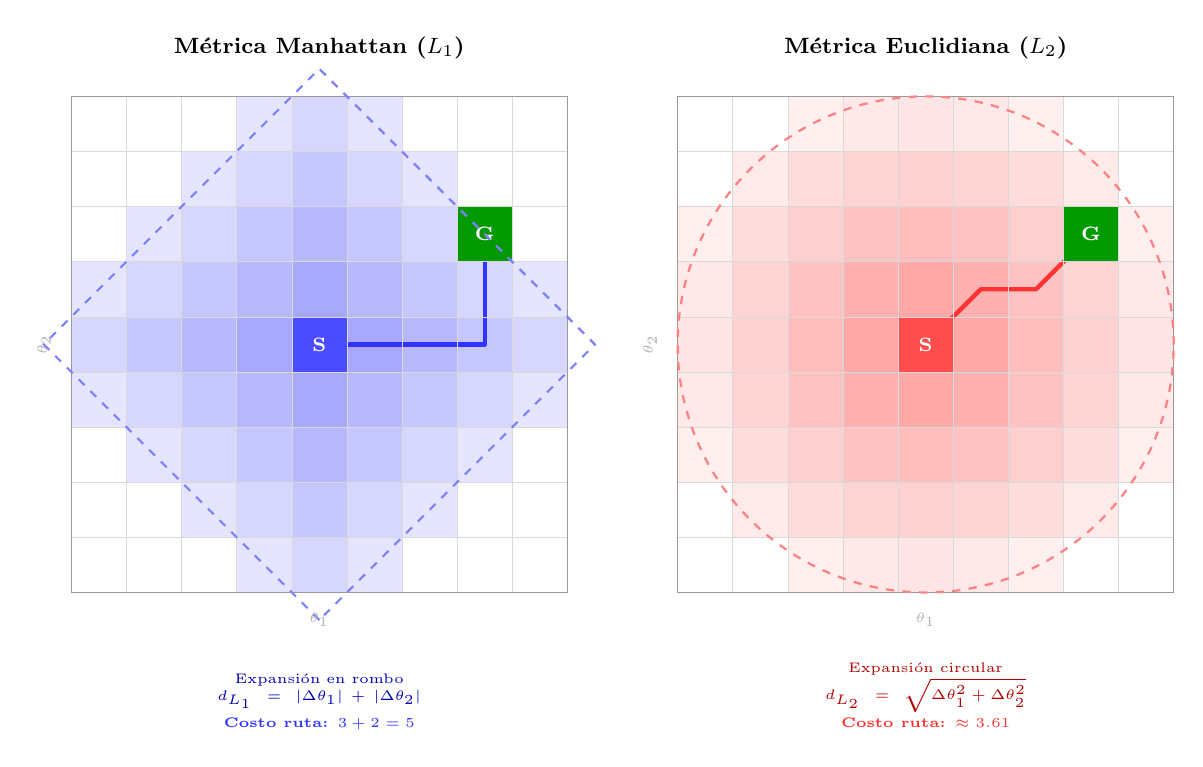
\begin{tikzpicture}[>=stealth, scale=0.7, every node/.style={font=\small}]

% Tamaño de la rejilla
\def\gridsize{9}
% Centro del inicio: celda (4,4), punto medio (4.5,4.5)
% Objetivo: celda (7,6), punto medio (7.5,6.5)

% =============================================
% PANEL IZQUIERDO: Métrica Manhattan (L1)
% =============================================
\begin{scope}[shift={(-6,0)}]
    \node[anchor=south, font=\bfseries\footnotesize] at (4.5, 9.5) {Métrica Manhattan ($L_1$)};
    
    % Rejilla de fondo
    \draw[gray!20, very thin] (0,0) grid (\gridsize,\gridsize);
    
    % Nodos expandidos en forma de rombo (diamante)
    % Centro en celda (4,4). Distancia Manhattan a G(7,6) = |7-4|+|6-4| = 5
    \foreach \x in {0,...,8} {
        \foreach \y in {0,...,8} {
            \pgfmathsetmacro{\mdist}{abs(\x-4) + abs(\y-4)}
            \pgfmathsetmacro{\opac}{max(0, min(35, 40 - 6*\mdist))}
            \ifdim \mdist pt < 5.5pt
                \fill[blue!\opac!white] (\x,\y) rectangle ++(1,1);
            \fi
        }
    }
    
    % Ruta Manhattan: S(4,4) → derecha hasta (7,4) → arriba hasta (7,6) → G
    \draw[blue!80, ultra thick, ->, line cap=round, line join=round] 
        (4.5,4.5) -- (7.5,4.5) -- (7.5,6.5);
    
    % Nodo central (inicio)
    \fill[blue!70] (4,4) rectangle ++(1,1);
    \node[font=\scriptsize\bfseries, white] at (4.5,4.5) {S};
    
    % Nodo objetivo
    \fill[green!60!black] (7,6) rectangle ++(1,1);
    \node[font=\scriptsize\bfseries, white] at (7.5,6.5) {G};
    
    % Redibujar rejilla
    \draw[gray!30, very thin] (0,0) grid (\gridsize,\gridsize);
    \draw[black!40, thin] (0,0) rectangle (\gridsize,\gridsize);
    
    % Contorno del rombo (radio 5, centrado en 4.5,4.5)
    \draw[blue!50, thick, dashed] 
        (4.5,-0.5) -- (-0.5,4.5) -- (4.5,9.5) -- (9.5,4.5) -- cycle;
    
    % Etiquetas de ejes
    \node[font=\tiny, gray!60] at (4.5,-0.5) {$\theta_1$};
    \node[font=\tiny, gray!60, rotate=90] at (-0.5,4.5) {$\theta_2$};
    
    % Anotación
    \node[anchor=north, font=\tiny, text=blue!70!black, text width=4cm, align=center] at (4.5, -1.3) {Expansión en rombo\\$d_{L_1} = |\Delta\theta_1| + |\Delta\theta_2|$};
    
    % Costo de la ruta
    \node[anchor=north, font=\tiny\bfseries, text=blue!80] at (4.5, -2.1) {Costo ruta: $3 + 2 = 5$};
\end{scope}

% =============================================
% PANEL DERECHO: Métrica Euclidiana (L2)
% =============================================
\begin{scope}[shift={(5,0)}]
    \node[anchor=south, font=\bfseries\footnotesize] at (4.5, 9.5) {Métrica Euclidiana ($L_2$)};
    
    % Rejilla de fondo
    \draw[gray!20, very thin] (0,0) grid (\gridsize,\gridsize);
    
    % Nodos expandidos en forma circular
    % Centro en celda (4,4). Distancia Euclidiana a G(7,6) = sqrt(9+4) ≈ 3.61
    \foreach \x in {0,...,8} {
        \foreach \y in {0,...,8} {
            \pgfmathsetmacro{\edist}{sqrt((\x-4)^2 + (\y-4)^2)}
            \pgfmathsetmacro{\opac}{max(0, min(35, 42 - 8*\edist))}
            \ifdim \edist pt < 4.5pt
                \fill[red!\opac!white] (\x,\y) rectangle ++(1,1);
            \fi
        }
    }
    
    % Ruta Euclidiana: más directa (diagonal)
    \draw[red!80, ultra thick, ->, line cap=round, line join=round] 
        (4.5,4.5) -- (5.5,5.5) -- (6.5,5.5) -- (7.5,6.5);
    
    % Nodo central (inicio)
    \fill[red!70] (4,4) rectangle ++(1,1);
    \node[font=\scriptsize\bfseries, white] at (4.5,4.5) {S};
    
    % Nodo objetivo
    \fill[green!60!black] (7,6) rectangle ++(1,1);
    \node[font=\scriptsize\bfseries, white] at (7.5,6.5) {G};
    
    % Redibujar rejilla
    \draw[gray!30, very thin] (0,0) grid (\gridsize,\gridsize);
    \draw[black!40, thin] (0,0) rectangle (\gridsize,\gridsize);
    
    % Contorno del círculo (radio ≈ 4.5, centrado en 4.5,4.5)
    \draw[red!50, thick, dashed] (4.5,4.5) circle (4.5);
    
    % Etiquetas de ejes
    \node[font=\tiny, gray!60] at (4.5,-0.5) {$\theta_1$};
    \node[font=\tiny, gray!60, rotate=90] at (-0.5,4.5) {$\theta_2$};
    
    % Anotación
    \node[anchor=north, font=\tiny, text=red!70!black, text width=4cm, align=center] at (4.5, -1.1) {Expansión circular\\$d_{L_2} = \sqrt{\Delta\theta_1^2 + \Delta\theta_2^2}$};
    
    % Costo de la ruta
    \node[anchor=north, font=\tiny\bfseries, text=red!80] at (4.5, -2.1) {Costo ruta: $\approx 3.61$};
\end{scope}

\end{tikzpicture}
